\documentclass[10pt]{article}
\usepackage{amsmath}
\usepackage[forpaper,pointsonboth,nototals,
nosolutions,allowrandomize
]{eqexam}



\usepackage{chemformula}
\usepackage[version=3]{mhchem}
\usepackage{varwidth}
\usepackage[utf8]{inputenc}
\usepackage[T1]{fontenc}
\usepackage[version=3]{mhchem}
\usepackage{booktabs}
\usepackage{paralist}
\usepackage{framed}
\usepackage{setspace}
\usepackage[spanish]{babel} 
\usepackage[left=2.85cm,top=2.5cm,right=2.85cm,bottom=1.25cm]{geometry}
\usepackage{tikz}
\usepackage{pgfplots}

\spanishdecimal{,}
%\usepackage{times}
%\usepackage{newcent}
%\usepackage{palatino}
%\usepackage{bookman}

\pointLabel{punto}
\pointsLabel{puntos}
\ptLabel{pt.}            % singular form
\ptsLabel{{pts.}}
\eachLabel{\tiny{apdo.}}
\renewcommand\itemPTsTxt[1]{{\footnotesize $#1$ pts}}
%%%%%%%%%%%%%%%%%%%%%%%%%%%%%%%%%%%%%%%%%%%%%%%%%
%%%%%%%%%%%%%%%%%%%%%%%%%%%%%%%%%%%%%%%%%%%%%%%%%
%%%%%%%%%%%%%%%%%%%%%%%%%%%%%%%%%%%%%%%%%%%%%%%%%
%%%%%%%%%%%%%%%%%%%%%%%%%%%%%%%%%%%%%%%%%%%%%%%%%

\begin{document}

\vspace*{-2.7cm}
\noindent\rule{1.05\textwidth}{0,4pt}
%Tipo examen y curso, Evaluacion
\noindent\makebox[1.05\linewidth]{{\bf{\small {Control-1 / 3º de ESO S}}}\hfill {\bf{\small{Segunda Evaluación}}}} 
\vspace{-0,35cm}
\noindent\makebox[1.05\linewidth]{{\bf{\scriptsize{Diversidad de la materia\ldots}}}\hfill\ {\bf{\scriptsize 17 de Junio de 2015}}}\vspace{0,65cm}
\noindent \makebox[1.05\linewidth]{Nombre\dotfill}\vspace{-0,25cm}
\noindent\rule{1.05\textwidth}{0,4pt}
\vspace*{-1.5cm}
%%%%%%%%%%%%%%%%%%%%%%%%%%%%%%%%%%%%%%%%%%%%%%%%%
%%%%%%%%%%%%%%%%%%%%%%%%%%%%%%%%%%%%%%%%%%%%%%%%%

\makeatletter
% \eqemargin is the minimum distance to the left margin, plus \marginparsep.
% I've removed \marginparsep to get the minimal positioning. You can insert
% additional spacing, such as 3pt+\eqemargin
\renewcommand{\eqleftmargin}[2]{\makebox[0pt][r]{\marginpointtext{#1}{#2}%
    \setlength{\@tempdima}{\eqemargin}%
%    \setlength{\@tempdima}{\marginparsep+\eqemargin}%
    \hspace*{\@tempdima}}}
% important to execute this after the redefinition
%\PointsOnLeft
\makeatother
\lhead{}
\chead{}
\rhead{}
%%%%%%%%%%%%%%%%%%%%%%%%%%%%%%%%%%%%%%%%%%%%%%%%%
%%%%%%%%%%%%%%%%%%%%%%%%%%%%%%%%%%%%%%%%%%%%%%%%%
%%%%%%%%%%%%%%%%%%%%%%%%%%%%%%%%%%%%%%%%%%%%%%%%%
%%%%%%%%%%%%%%%%%%%%%%%%%%%%%%%%%%%%%%%%%%%%%%%%%

\begin{exam}{Part1}
\forceNoColor
%\useFillerLines
\useFillerDefault
%\fillTypeHRule
%\fillTypeDefault
%\fillTypeDashLine
\fillTypeDots
\eqWriteLineColor{blue}
\eqWLSpacing{18pt}
\vspace*{1cm} \begin{problem*}[10ea] 
El coeficiente de rozamiento entre $m_1$ y el plano sobre el que desliza es de $\mu=0.3$ y calcula: \\
\begin{minipage}{\linewidth}
\begin{varwidth}{0.5\linewidth}
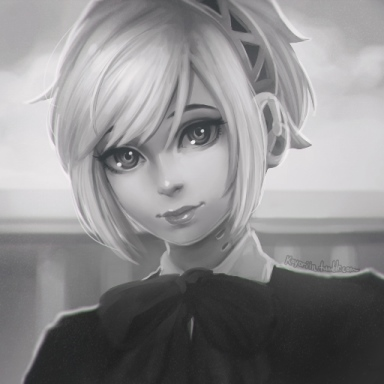
\includegraphics[scale=0.4]{grafico5.jpg}
\end{varwidth}\hfill
\begin{varwidth}{0.5\linewidth}
\begin{parts}
\item  Representa las fuerzas implicadas en cada una de las masas.
\item ¿Cuánto debe valer $m_1$, si en 2 s ha recorrido 2 m sobre el plano?
\item Calcula las tensiones de las cuerdas.
\end{parts}
\end{varwidth}
\end{minipage}
\end{problem*}\vfill
\hrule
\vspace*{0.2cm}
\noindent{\footnotesize\emph{{La puntuación total del examen es de \summaryPointTotal\ puntos.}}}
\end{exam} 
\end{document}

